\documentclass[10pt,]{article}
\usepackage{lmodern}
\usepackage{amssymb,amsmath}
\usepackage{ifxetex,ifluatex}

% BDC stuff
\usepackage{wrapfig}
\usepackage[font=footnotesize,labelfont=bf]{caption}
\renewcommand{\figurename}{Fig.}
\usepackage{titlesec}                                                           
\titleformat{\section}{\normalfont\large\bfseries}{}{0em}{}                     
\titleformat{\subsection}{\normalfont\large\bfseries}{}{0em}{}                  
\titleformat{\subsubsection}{\normalfont\normalsize\bfseries}{}{0em}{}          
\titlespacing{\section}{0pt}{*1}{*1}                                            
\titlespacing{\subsection}{0pt}{*1}{*-0.8}                                      
\titlespacing{\subsubsection}{0pt}{*1}{*-0.8}

\usepackage{fixltx2e} % provides \textsubscript
\ifnum 0\ifxetex 1\fi\ifluatex 1\fi=0 % if pdftex
  \usepackage[T1]{fontenc}
  \usepackage[utf8]{inputenc}
\else % if luatex or xelatex
  \ifxetex
    \usepackage{mathspec}
    \usepackage{xltxtra,xunicode}
  \else
    \usepackage{fontspec}
  \fi
  \defaultfontfeatures{Mapping=tex-text,Scale=MatchLowercase}
  \newcommand{\euro}{€}
\fi
% use upquote if available, for straight quotes in verbatim environments
\IfFileExists{upquote.sty}{\usepackage{upquote}}{}
% use microtype if available
\IfFileExists{microtype.sty}{%
\usepackage{microtype}
\UseMicrotypeSet[protrusion]{basicmath} % disable protrusion for tt fonts
}{}
\usepackage[margin=0.72in]{geometry}
\usepackage{graphicx}
\makeatletter
\def\maxwidth{\ifdim\Gin@nat@width>\linewidth\linewidth\else\Gin@nat@width\fi}
\def\maxheight{\ifdim\Gin@nat@height>\textheight\textheight\else\Gin@nat@height\fi}
\makeatother
% Scale images if necessary, so that they will not overflow the page
% margins by default, and it is still possible to overwrite the defaults
% using explicit options in \includegraphics[width, height, ...]{}
\setkeys{Gin}{width=\maxwidth,height=\maxheight,keepaspectratio}
\ifxetex
  \usepackage[setpagesize=false, % page size defined by xetex
              unicode=false, % unicode breaks when used with xetex
              xetex]{hyperref}
\else
  \usepackage[unicode=true]{hyperref}
\fi
\hypersetup{breaklinks=true,
            bookmarks=true,
            pdfauthor={Brian D. Connelly and Caroline Turner},
            pdftitle={Evolution of Cooperation through Niche Construction Feedback},
            colorlinks=true,
            citecolor=blue,
            urlcolor=blue,
            linkcolor=magenta,
            pdfborder={0 0 0}}
\urlstyle{same}  % don't use monospace font for urls
\setlength{\parindent}{0pt}
\setlength{\parskip}{6pt plus 2pt minus 1pt}
\setlength{\emergencystretch}{3em}  % prevent overfull lines
\setcounter{secnumdepth}{0}

\date{}

\begin{document}

\section{Evolution of Cooperation through Niche Construction
Feedback}\label{evolution-of-cooperation-through-niche-construction-feedback}

Cooperative behaviors are common across all branches of the tree of
life. Insects divide labor within their colonies, plants and soil
bacteria exchange essential nutrients, birds care for others' young, and
the trillions of cells in the human body restrain their growth and
coordinate to provide vital functions. Each instance of cooperation
presents an evolutionary challenge: How can individuals that sacrifice
their own well-being to help others avoid subversion by those that do
not? Over time, we would expect these \emph{defectors} to rise in
abundance at the expense of others, eventually driving cooperators---and
perhaps the entire population---to extinction.

\begin{wrapfigure}{R}{0.28\textwidth}                                   
    \centering                                                          
    \vspace{-2.2em}
    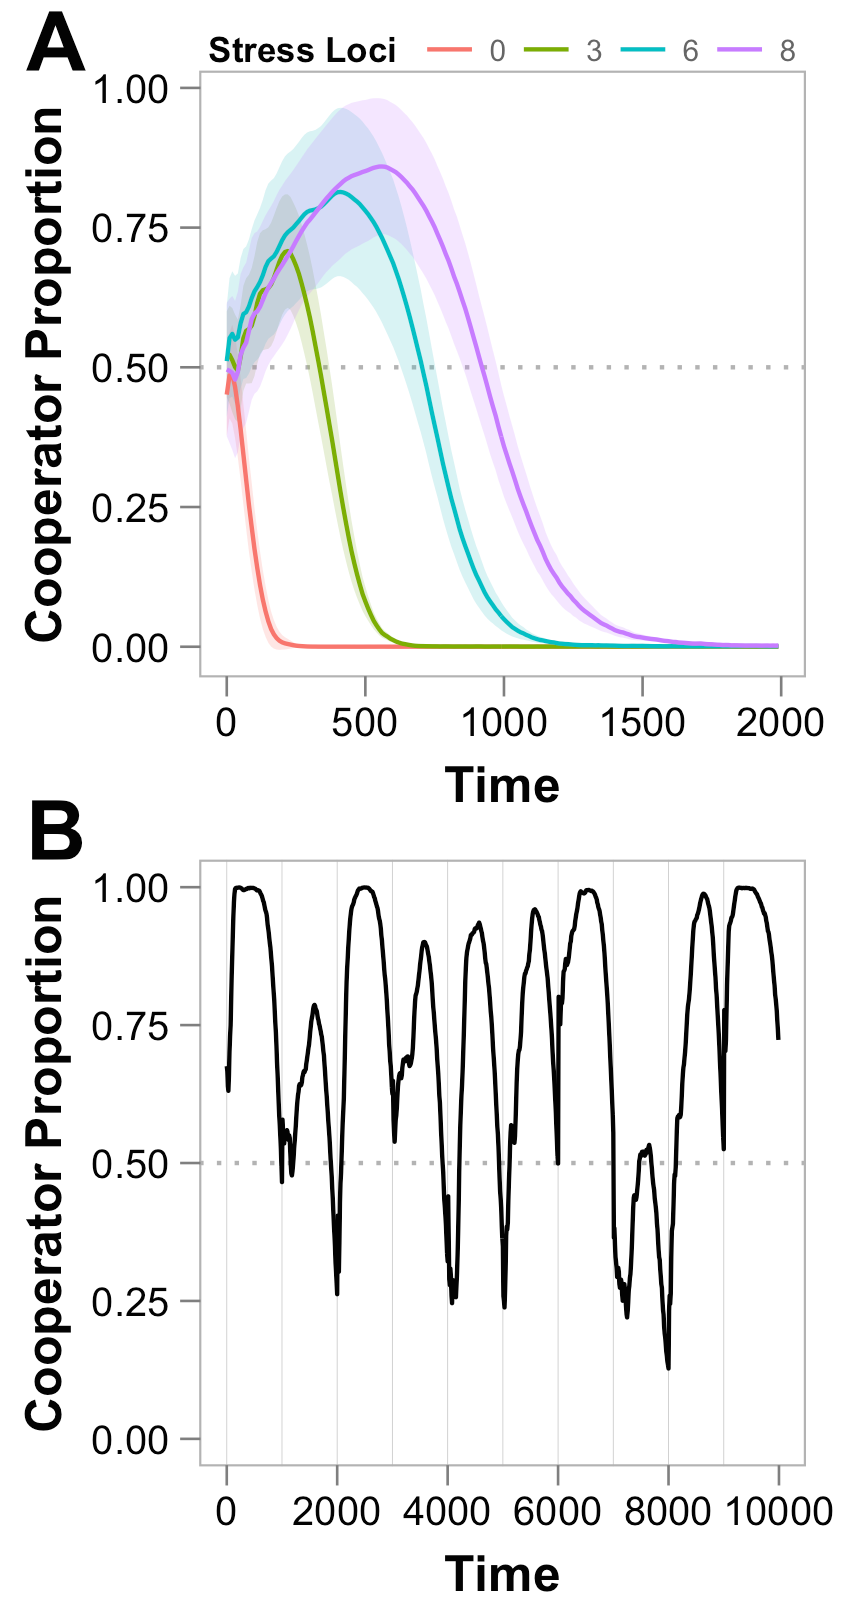
\includegraphics[width=0.278\textwidth]{figures/Figure1all} 
    \caption{(\textbf{A}) Through ``genetic niche hiking'', cooperators
    outrun defectors by association with non-social adaptations that
    compensate for the cost of cooperation. Colored lines represent
    different opportunities for adaptation (or ``stress loci'' in our
    model). Once defectors become equally adapted, however, they quickly
    drive cooperators to extinction. (\textbf{B}) When environmental change
    is frequent (here every 1,000 cycles), the continual potential for
    adaptation allows cooperators to persist indefinitely.}
    \label{fig1}
    \vspace{-2em}
\end{wrapfigure} 

Several factors can defer this potential \emph{tragedy of the
commons}\textsuperscript{1--4}. For example, cooperators must benefit more from
the cooperative act than others. This can occur when cooperators are clustered
together in spatially-structured populations\textsuperscript{5--7} or when
cooperators use communication\textsuperscript{8,9} or other
cues\textsuperscript{10--12} to cooperate conditionally with kin.
Interestingly, cooperation can also be bolstered by genetic linkage with
self-benefitting traits\textsuperscript{13--15}, setting the stage for an
``adaptive race'' in which cooperators and defectors vie for the first
highly-beneficial non-social adaptation\textsuperscript{16,17}. We recently
showed that cooperators can gain a substantial leg up on defectors in an
adaptive race when the cooperative behavior increases local population density,
thus increasing the likelihood of acquiring beneficial non-social mutations (in
prep.).  Nevertheless, this advantage is fleeting (Fig. 1A). As soon as the
opportunities for adaptation are exhausted, cooperators are once again at a
disadvantage against defectors. As shown in Fig. 1B, however, cooperation can
be maintained indefinitely when frequent environmental changes produce a stream
of non-social adaptive opportunities. Although natural organisms typically find
themselves in changing environments, cooperators may not be able to rely on the
the environment to provide sufficient adaptive opportunities for their
long-term survival.

Previous studies on the evolution of cooperation have have typically
neglected one potentially major determinant of evolutionary outcomes:
environmental change brought about by the organisms themselves. Through
their metabolism, their interactions with others, and even through their
deaths, organisms constantly modify their environment. These changes can
produce evolutionary feedback loops in which environmental change alters
selection, which, in turn, alters phenotypes and their corresponding
effects on the environment\textsuperscript{18}. \textbf{This research
will reveal how environmental change brought about by organisms, or \emph{niche
construction}, affects the evolution of cooperation.} First, we will
explore how selective feedbacks influence evolution as populations
construct their environment. We then widen our scope to include
scenarios where the environment itself is biotic, such as when symbiont
populations modify their host.

Because this research requires a level of control over both population
and environment that would be difficult to attain even with
well-characterized systems, we employ computational modeling for these
initial studies. However, we expect that the results gained through this
project will be instrumental in designing future microbial experiments.
We first describe the model that will be developed and then detail how
it will be used to study the effects of niche construction on the
evolution of cooperation in two contexts.

\textbf{Model Description}  In our proposed agent-based model, each individual
has a genotype of length \(L+1\). A binary allele at the first locus determines
whether or not the individual is a cooperator, which carries cost \(c\). The
remaining \(L\) loci are \emph{stress loci}, and are each occupied by a \(0\)
or an integer from the set \(A=\{1, \ldots, a_{max}\}\), where \(a_{max}\) is
the number of possible alleles. These alleles represent adaptations to the
environment, and the number of loci determines the number of possible
adaptations. All non-zero alleles carry fitness benefit \(\delta\).  Organisms
also influence their environment, which can feed back to influence selection.
We model this as a form of frequency dependent selection.  Specifically, the
selective value of allele $a$ at locus $i$ increases with the proportion of the
population that has allele $a-1$ (modulo $A$) at locus $i-1$.  The slope of
this increase is $\epsilon$ (which gauges the intensity of niche construction).
As a consequence of this form of frequency dependence, genotypes with
sequentially increasing allelic states will tend to evolve.  Because mutations
are random, as described below, each population will evolve sequences that
start with different allelic states. These different sequences represent the
unique niches constructed by populations.

We observe the evolutionary process in a metapopulation of \(N\)
populations, which are initiated with non-adapted individuals and
cooperator proportion \(p_0\). Each population grows to capacity
\(S_{min} + p (S_{max} - S_{min})\), where \(p\) is the proportion of
cooperators in that population. After growth, mutations alter the
allelic state at stress loci and the cooperation locus with
probabilities \(\mu_{s}\) and \(\mu_{c}\), respectively. Individuals
then migrate to a randomly chosen neighbor patch at rate \(m\). Finally,
populations are thinned to proportion \(d\) to accommodate the next
cycle of growth.

\begin{wrapfigure}{R}{0.28\textwidth}
    \centering
    \vspace{-1em}
    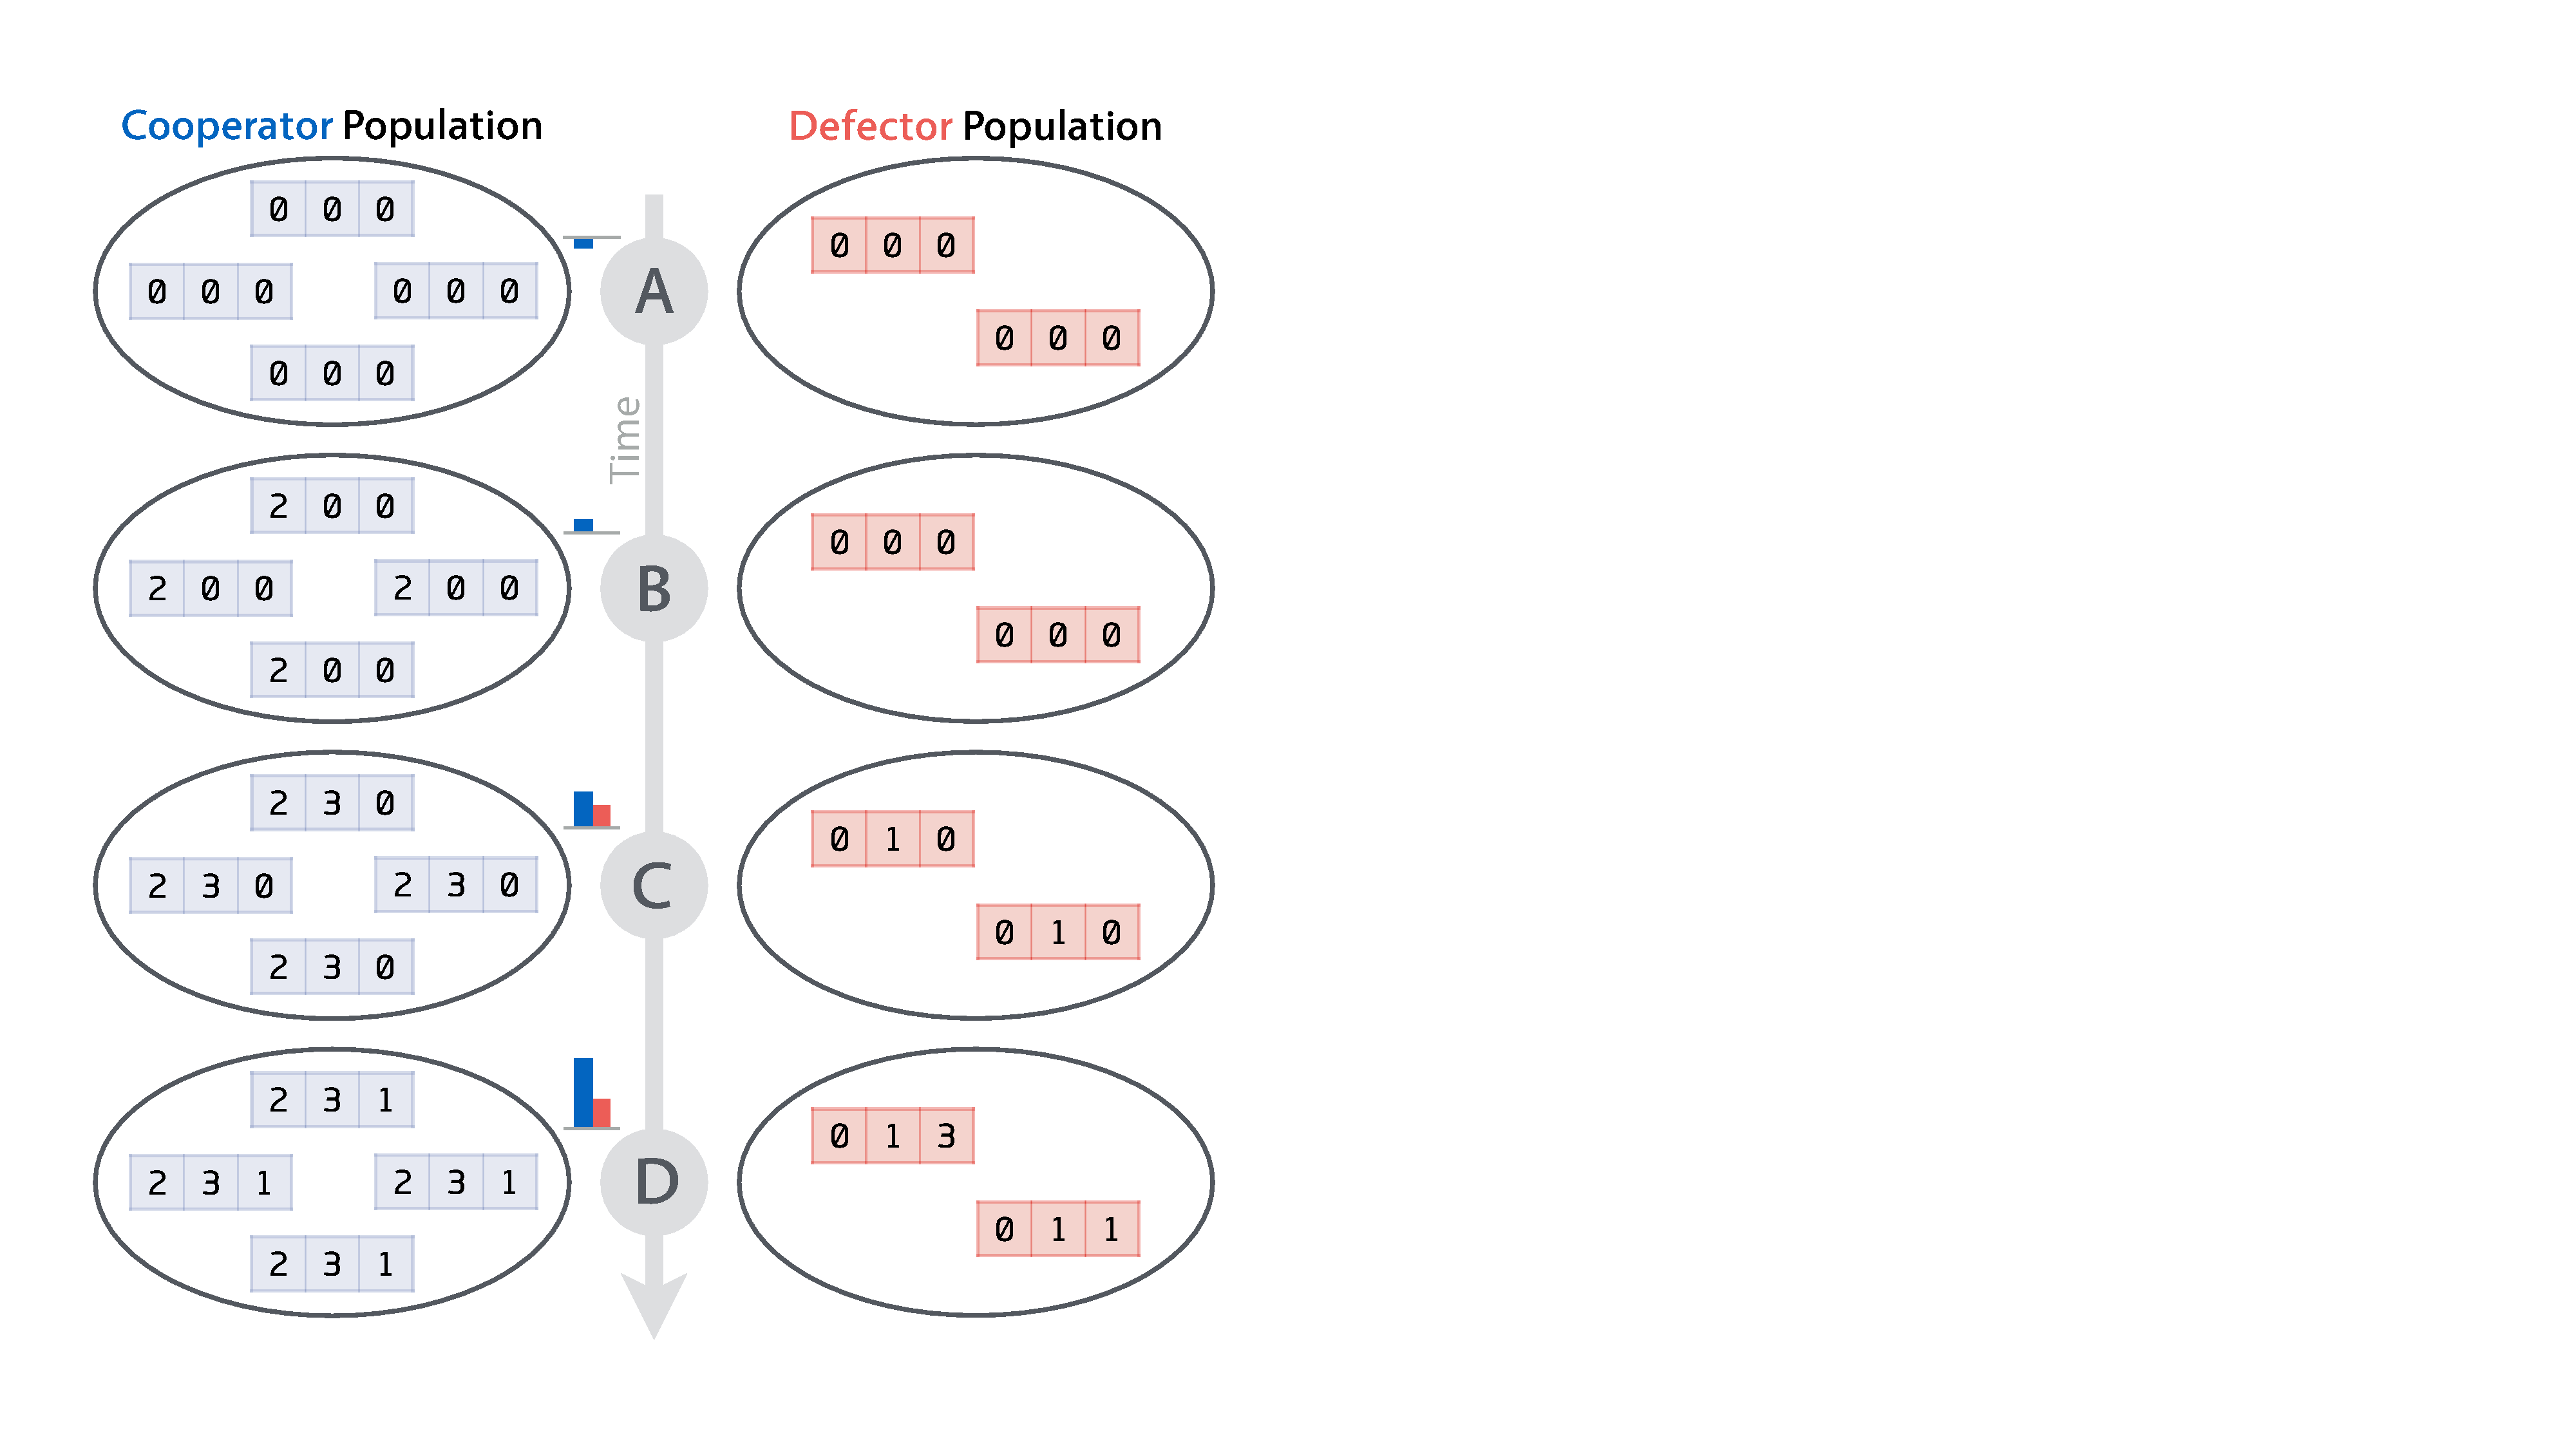
\includegraphics[width=0.279\textwidth]{figures/diagram1} 
    \caption{\textbf{Model Overview:} For simplicity, we consider two clonal
populations. (\textbf{A}) Because public good production is costly, the
cooperator population has lower fitness relative to the defector
population, as shown in the bar graph. However, these public goods enable
the cooperator population to be larger. (\textbf{B}) As a result, the
cooperator population acquires beneficial mutations more quickly,
allowing cooperator fitness to surpasses that of the ancestral defector
(bar graph baseline). (\textbf{C}) Selection favors alleles at adjacent
loci that form sequences, offering a further boost to cooperators. Here,
there 3 possible alleles, so allelic state 1 follows 3. (\textbf{D}) The
cooperator patch now favors individuals with allelic state \(2,3,1\).}
    \label{fig2}
\end{wrapfigure} 


\subsection{Can Niche Construction Feedbacks Sustain the Evolution of
Cooperation?}\label{can-niche-construction-feedbacks-sustain-the-evolution-of-cooperation}

As illustrated in Fig. 2, we will first explore how selective feedbacks affect
the evolution of cooperative public goods production. In our model, public
goods enable populations to reach greater densities (\(S_{max} > S_{min}\)).
This increase in growth provides larger populations with more mutational
opportunities to gain non-social adaptations. Importantly, as populations
adapt, they alter selection at their patch. Using our model (varying parameters
\(\epsilon\) and \(a_{max}\)), we will explore how the degree to which
individuals construct their environments affects evolutionary trajectories and
outcomes. Aside from providing adaptive opportunity, niche construction may
diminish the threat of invasion by immigrant defectors (Fig. 3). We also hope
to gain an understanding of how emigration allows populations to effectively
export their environment, and whether this benefits cooperators, whose larger
populations produce more migrants.


\begin{wrapfigure}{R}{0.28\textwidth}
%    \centering
    \vspace{18.5em}
    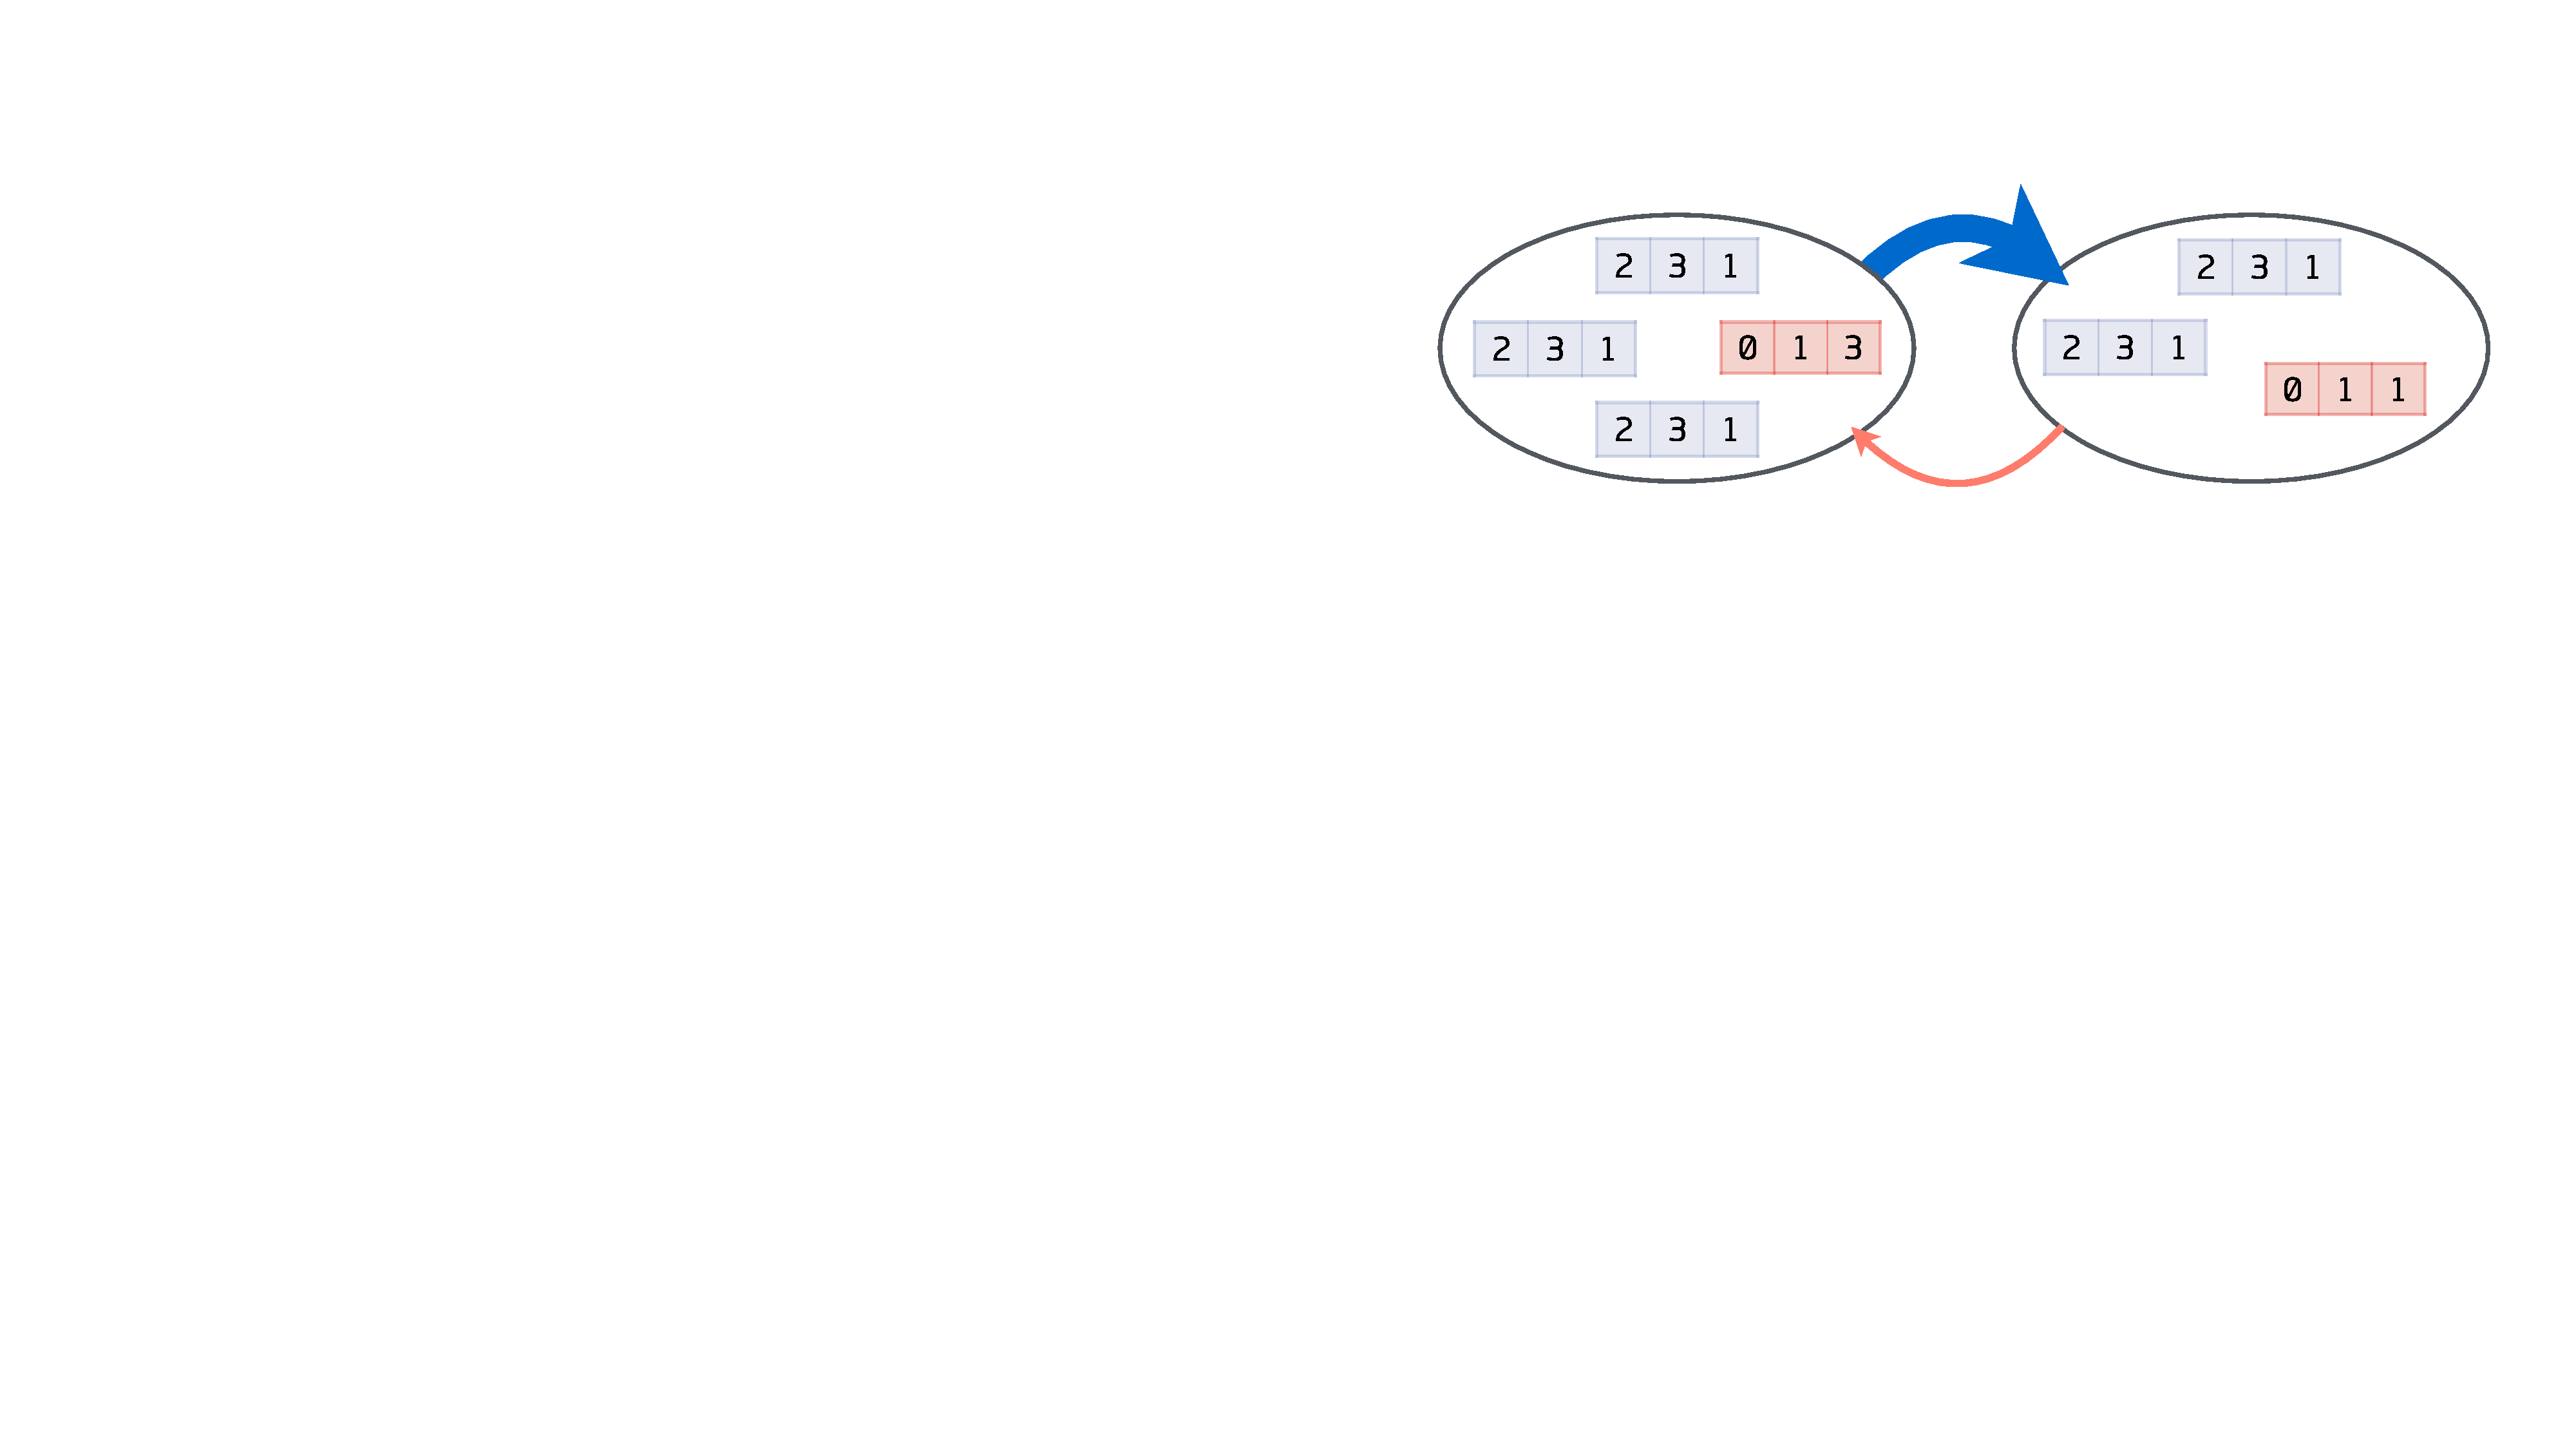
\includegraphics[width=0.279\textwidth]{figures/diagram2}
\caption{Migration reveals two key effects of niche construction. First,
when immigrating to the cooperator patch (left), defectors will be at a
disadvantage against cooperators, which are more adapted to their
environment (2, 3, 1). Second, the larger group of
cooperators that emigrate to the defector population (right) will
strongly affect selection at the defector patch, effectively
``exporting'' their niche.}
    \label{fig2}
    \vspace{-15em}
\end{wrapfigure} 


\subsection{How do Selective Feedbacks affect Host-Symbiont
Co-Evolution?}\label{how-do-selective-feedbacks-affect-host-symbiont-co-evolution}

For our first aim, the state of the environment is implicit, depending
entirely on the composition of the population. However, the environment
is often itself a biological entity, which can produce additional
evolutionary feedbacks. These feedbacks are certainly present in
infections and the human microbiome, where bacterial behaviors greatly
affect host fitness. As the host population changes, so too will
selection on their symbiont populations. Here, evolutionary outcomes
depend greatly on the degree of shared interest between the host and
symbiont. For example, the cooperative production of virulence factors
by the human pathogen \emph{P. aeruginosa} in lung infections is harmful
to those with cystic fibrosis. Conversely, cooperative light production
by \emph{A. fischeri} is vital for the survival of its host, the
Hawaiian bobtail squid.

To address how feedbacks from niche construction affect social evolution in
host-symbiont systems, we will extend our model to include selection and
replication at the host level. Here, patches will be replaced by replicating
hosts. Each host will have a genotype, and their fitness will depend both on
this genotype and the genotypes in their symbiont populations. We can control
this relationship by altering the symmetry of the fitness effects of a match
between host and symbiont genotypes. If a match improves the fitness of both
players simultaneously, the relationship is mutualistic. If a match improves
fitness of the symbiont, but not the host, then the relationship is
antagonistic (e.g., the symbiont is a parasite). By altering such features, we
will be able to observe how host-symbiont co-evolution differs with
\emph{positive} and \emph{negative niche construction}. Using this model, we
can also explore how co-evolution differs when symbiont populations are
transferred vertically or horizontally.

\vspace{-0.5em}
\subsection{Summary}\label{summary}

Using a model of public goods production, this project will explore how
the selective feedbacks that result from niche construction affect the
evolution of cooperative behaviors from both a population-level and a
host-symbiont perspective. Both investigators are currently studying the
relationship between ecology and evolution, and the results from this
study will inform future microbial experiments in their labs. It was
recently suggested that this niche construction perspective will be
critical for improving our understanding of viral
evolution\textsuperscript{19} and evolution in co-infecting
parasites\textsuperscript{20}. We believe it may play the same role in
understanding the evolution of cooperative behaviors.

\clearpage

\section*{References}\label{references}
\addcontentsline{toc}{section}{References}

1. Hardin, G. The tragedy of the commons. \emph{Science} \textbf{162,}
1243--1248 (1968).

2. Hamilton, W. D. The genetical evolution of social behaviour I \& II.
\emph{Journal of Theoretical Biology} \textbf{7,} 1--52 (1964).

3. Nowak, M. A. Five rules for the evolution of cooperation.
\emph{Science} \textbf{314,} 1560--1563 (2006).

4. West, S. A., Griffin, A. S. \& Gardner, A. Evolutionary explanations
for cooperation. \emph{Current Biology} \textbf{17,} R661--R672 (2007).

5. Kuzdzal-Fick, J. J. \emph{et al.} High relatedness is necessary and
sufficient to maintain multicellularity in Dictyostelium. \emph{Science}
\textbf{334,} 1548--1551 (2011).

6. Fletcher, J. A. \& Doebeli, M. A simple and general explanation for
the evolution of altruism. \emph{Proceedings of the Royal Society B:
Biological Sciences} \textbf{276,} 13--19 (2009).

7. Nadell, C. D., Foster, K. R. \& Xavier, J. B. Emergence of spatial
structure in cell groups and the evolution of cooperation. \emph{PLoS
Computational Biology} \textbf{6,} e1000716 (2010).

8. Darch, S. E. \emph{et al.} Density-dependent fitness benefits in
quorum-sensing bacterial populations. \emph{Proceedings of the National
Academy of Sciences} \textbf{109,} 8259--8263 (2012).

9. Brown, S. P. \& Johnstone, R. A. Cooperation in the dark: Signalling
and collective action in quorum-sensing bacteria. \emph{Proceedings of
the Royal Society of London B: Biological Sciences} \textbf{268,}
961--965 (2001).

10. Gardner, A. \& West, S. A. Greenbeards. \emph{Evolution}
\textbf{64,} 25--38 (2010).

11. Sinervo, B. \emph{et al.} Self-recognition, color signals, and
cycles of greenbeard mutualism and altruism. \emph{Proceedings of the
National Academy of Sciences} \textbf{103,} 7372--7377 (2006).

12. Veelders, M. \emph{et al.} Structural basis of flocculin-mediated
social behavior in yeast. \emph{Proceedings of the National Academy of
Sciences} \textbf{107,} 22511--22516 (2010).

13. Dandekar, A. A., Chugani, S. \& Greenberg, E. P. Bacterial quorum
sensing and metabolic incentives to cooperate. \emph{Science}
\textbf{338,} 264--266 (2012).

14. Asfahl, K. L. \emph{et al.} Non-social adaptation defers a tragedy
of the commons in Pseudomonas aeruginosa quorum sensing. \emph{The ISME
Journal} (2015).
doi:\href{http://dx.doi.org/10.1038/ismej.2014.259}{10.1038/ismej.2014.259}

15. Foster, K. \emph{et al.} Pleiotropy as a mechanism to stabilize
cooperation. \emph{Nature} \textbf{431,} 693--696 (2004).

16. Waite, A. J. \& Shou, W. Adaptation to a new environment allows
cooperators to purge cheaters stochastically. \emph{Proceedings of the
National Academy of Sciences} \textbf{109,} 19079--19086 (2012).

17. Morgan, A. D. \emph{et al.} Selection on non-social traits limits
the invasion of social cheats. \emph{Ecology Letters} \textbf{15,}
841--846 (2012).

18. Odling-Smee, F. J., Laland, K. N. \& Feldman, M. W. \emph{Niche
construction: The neglected process in evolution}. (Princeton University
Press, 2003).

19. Hamblin, S. R., White, P. A. \& Tanaka, M. M. Viral niche
construction alters hosts and ecosystems at multiple scales.
\emph{Trends in Ecology \& Evolution} \textbf{29,} 594--599 (2014).

20. Hafer, N. \& Milinski, M. When parasites disagree: Evidence for
parasite-induced sabotage of host manipulation. \emph{Evolution} (2015).
doi:\href{http://dx.doi.org/10.1111/evo.12612}{10.1111/evo.12612}

\end{document}
